OpenCL (Open Computing Language) is a low-level API written in C/C++.
It is aimed for cross-platform computing and can be used for CPUs\footnote{Central Processing Unit} and GPUs, but also DSPs\footnote{Digital Signal Processor} and FPGAs\footnote{Field-programmable Gate Arrays}.

\begin{wrapfigure}{r}{0.31\textwidth}
	\centering
	\fbox{
		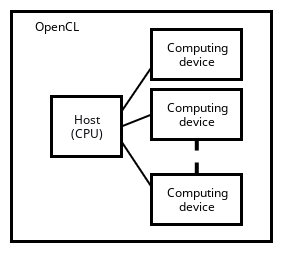
\includegraphics[width=0.3\textwidth]{figs/extra/opencl.png}
	}
	\caption{OpenCL concepts} 
	\label{fig:opencl}
\end{wrapfigure}

\noindent The core of OpenCL's programming model is that it views a computing system as a number computing devices that are attached to a host processor as shown in \autoref{fig:opencl}.
OpenCL enables parallel programming of heterogeneous systems and can be used to write and launch GPU kernels.
Many vendors such as Nvidia, AMD, Apple, Intel and Xilinx support OpenCL.
Using OpenCL enhances code portability, but at the expense of speed, since many optimizations are very platform dependent.

OpenCL's programming model reflects many of the same characteristics as in CUDA.
For instance, the memory model is very much alike where OpenCL's memory hierarchy defines four levels:
\begin{itemizeSmall}
	\item Global memory - shared by all devices with a high access latency.
	\item Read-only memory - smaller, low latency memory, where only the host CPU can write, while other computing devices only can read.
	\item Local memory - shared by a group of computing devices.
	\item Per-element private memory - corresponds to registers in each computing device.
\end{itemizeSmall}
Kernels are also written in a very similar way as in CUDA.
In general OpenCL programming resembles CUDA a lot.
Thus a transition from writing parallel programs in CUDA to OpenCL is somewhat straightforward since many of the concepts are the same.